\documentclass[aspectratio=169]{beamer}
\usetheme[language=ngerman,
titlepagelogo=logopolito,
bullet=circle,
pageofpages=of,
titleline=true,
color=blue
]{TorinoTh}

%\usepackage[ngerman]{babel}
%\usepackage[utf8]{inputenc}
\usepackage{tabularx}
\usepackage{booktabs}
\usepackage{multicol}
\usepackage{ulem}
\usepackage{makecell}

\addto{\captionsngerman}{%
  \renewcommand*{\contentsname}{Contents}
  \renewcommand*{\listfigurename}{Figures}
  \renewcommand*{\listtablename}{Tables}
  \renewcommand*{\figurename}{Fig.}	
  \renewcommand*{\tablename}{Tab.}
}

\newcommand{\tabitem}{~~\llap{\textbullet}~~}

\usepackage{color}
\usepackage{graphicx}
\usepackage{fancybox}

\usepackage{beamerthemesplit}
\usetheme[compress]{Heidelberg}
\definecolor{unirot}{rgb}{0.4,0.4,0.3} % babyblue 0,0.58,1
\usecolortheme[named=unirot]{structure}
%\setbeamercolor{alerted text}{fg=red}
\newcommand*\hilite[1]{\textcolor{red}{#1}}
%\def\hilite<#1>{%
  %\temporal<#1>{\color{black}}{\color{unirot}}%
               %{\color{gray}}}

\title[Light Transport Techniques for Tensor Field Visualization]{Light Transport Techniques for Tensor Field Visualization}
%\subtitle{}
\author[Sebastian Bek]{Sebastian Bek}
\date{\today}
\institute[Uni HD]{
Heidelberg University\\
Visual Computing Group (VCG)\\
Master's Thesis Presentation\\
Supervisors: Prof. Filip Sadlo, Dr. Susanne Krömker\\
%\color{unirot}{sebibek@gmail.com}}
}

%---------------------------------------%
%---------- RECURRING OUTLINE ----------%
% have this if you'd like a recurring outline
\AtBeginSection[]  % "Beamer, do the following at the start of every section"
{
\begin{frame}<beamer> 
\frametitle{Outline} % make a frame titled "Outline"
\tableofcontents[currentsection,hideallsubsections]  % show TOC and highlight current section
\end{frame}
}
%----------------------------------------


\begin{document}
\frame[plain]{\titlepage}
\frame{\frametitle{Outline}\tableofcontents[hideallsubsections]}

%========================================
%========================================

\section[Introduction]{Introduction}

\subsection[Introduction]{Motivation}

\frame{
\frametitle{{Motivation}}

\begin{itemize}
	\item visualization in general is needed to generate a more readable, explorable and intuitive representation
	\item tensor representations are needed to describe a directional distribution for each point in space, when:
	\begin{itemize}
	\item e.g. for vector fields: to describe the directionally dependent spatial gradient called Jacobian-matrix,
	\item e.g. for fluid and solid continuum mechanics: to describe a whole distribution of stresses
	\item e.g. for DT-MRI: diffusion tensor - magnetic resonance imaging: to describe the diffusion characteristics of water molecules within tissue
	\end{itemize}
\end{itemize}
} % END OF FRAME


\frame{
\frametitle{{Objectives}}

\begin{itemize}
	\item a light transport model (propagation scheme) following basic but crucial physical principles,
	\item application of this model for tensor field visualization interpreting tensors as light transmission properties,
	\item a FTLE (Finite-time Lyapunov exponents)-related approach called light transport gradient (LTG) for visualizing key structures, namely LCS (Lagrangian coherent structures) in 2D second-order tensor fields, and
	\item application of our approach to both synthetic and real data involving brain and heart datasets.
\end{itemize}

} % END OF FRAME
%----------------------------------------

\subsection[Introduction]{Related Work}

\frame{
\frametitle{{Related Work - Global Illumination Methods}}
\begin{columns}
\begin{column}{.5\textwidth}
\begin{itemize}
	\item Discrete Ordinates Method: discretizes RTE in both spatial and angular domain
	\bigskip
	\item Lattice-Boltzmann method: light propagation modeled as a diffusion process
	\bigskip
	\item Light Propagation Volumes: light exchanged between neighboring cells and stored locally in capacities
\end{itemize}
\end{column}
\begin{column}{.5\textwidth}
\begin{figure}[t]
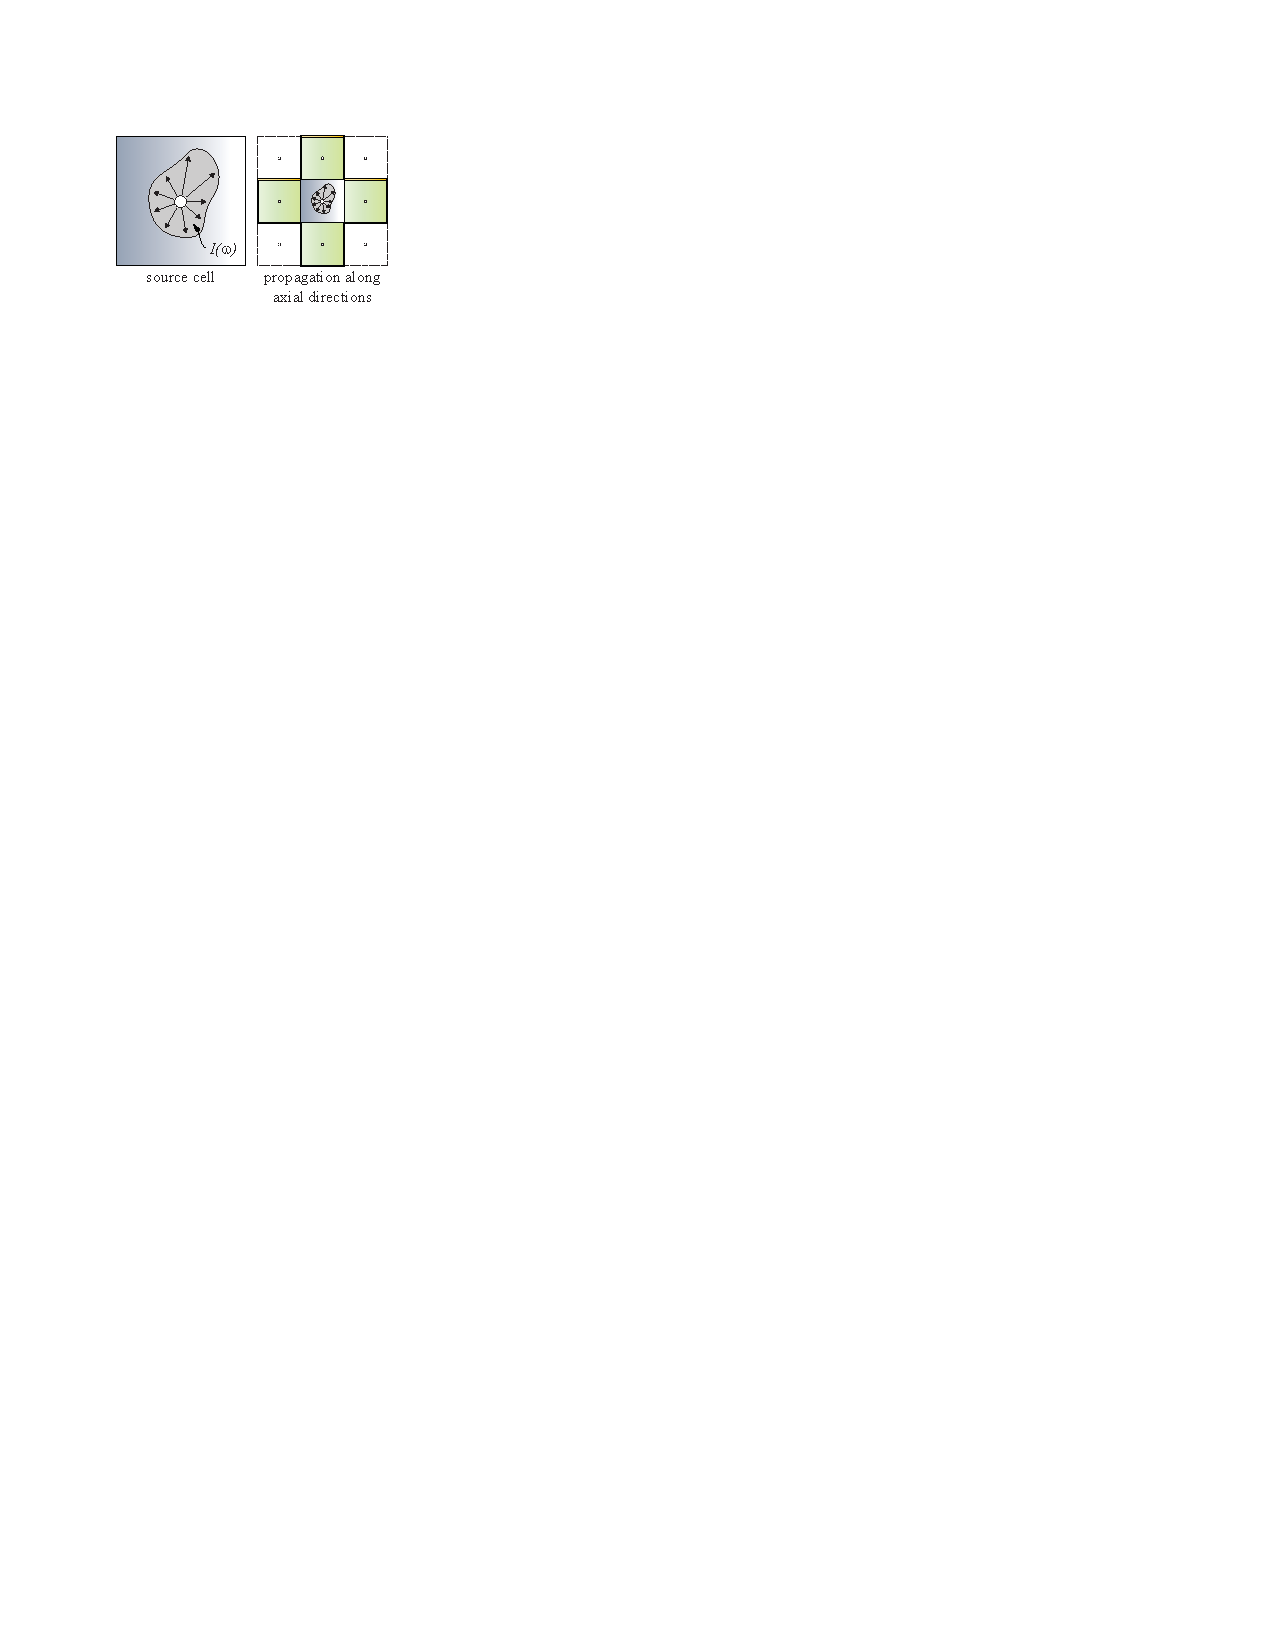
\includegraphics[width=0.5\textwidth]{LPV.pdf} 
\caption{Light Propagation Volumes,  \textit{Source: \textcircled{1}}}
\end{figure}
\end{column}
\end{columns}


} % END OF FRAME

\frame{
\frametitle{{Related Work - Symmetric Tensor Field Visualization}}

\begin{itemize}
	\item Glyphs: represent anisotropy with shape and orientation
	\item Tensor Field Lines (TFLs): follow the eigenvector along tensor field lines
	\item Tensorlines: introduce artificial inertia on TFLs to increase stability
	\item HyperLIC: use Line Integral Convolution from Vector Field Visualization on TFLs
	\item FTLE: exploit the gradient of the flow map of TFLs to generate an FTLE field
	\item Scalar Measures: tensor magnitude, diffusivity, fractional anisotropy, anisotropy coefficients (measures)
\end{itemize}


} % END OF FRAME

\frame{
\frametitle{{Related Work - Asymmetric Tensor Field Visualization}}

\begin{itemize}
	\item Dual Eigenvectors:
	\bigskip
	\item Pseudo Eigenvectors:
	\bigskip
	\item Scalar Measures: tensor magnitude, tensor mode, isotropy index
\end{itemize}


} % END OF FRAME
%----------------------------------------


%----------------------------------------

%======================================== END OF SECTION

\section[Fundamentals]{Fundamentals}
\subsection[Fundamentals]{Fundamentals}

\frame{
\frametitle{{Fundamentals}}

\begin{block}{\centering \textbf{Important Terms}}
\begin{align*}
	\text{prior (data) distribution}&: p_{data}=p_z(z)\sim z\\
	\text{generator function}&: G(z,\theta_g)\hskip 20pt \theta_g: \text{generator parameters}\\
	\text{discriminator function}&: D(x,\theta_d)\hskip 20pt \theta_d: \text{discriminator parameters}
\end{align*}\vskip 5pt
whereas $D(x)$ represents the propability that x is drawn from the training samples (prior data distribution) rather than $p_g$.

\end{block}
} % END OF FRAME

\frame{
\frametitle{{Mathematical Formulation}}


\begin{block}{\centering \textbf{Formal Definition}}
\textbf{Two-Player Minimax} (specific: zero-sum) game with value function $V(G,D)$:
\begin{align*}
	\min_G\max_D V(D,G) &=  \mathbb{E}_{x\sim p_{data}(x)}[\log D(x)] + \mathbb{E}_{z\sim p_z(z)}[\log (1-D(G(z))] \\
	&\Rightarrow \max V(D,G) = 0\hskip 30pt \min V(D,G) = -\infty
\end{align*}
outer loop: minimize $V(D,G)$ for $1$ step
 \  $\mid$ \
inner loop: maximize $V(D,G)$ for $k$ steps \vskip 3pt
$\rightarrow$ prevents the network from overfitting the training data\\
$\rightarrow$ stop when gradient of $G$ is very small $\Rightarrow$ slowly changing ($\ddot{G}\approx 0$)
\end{block}
} % END OF FRAME

\frame{
\frametitle{{Precautions}}

\begin{block}{\centering \textbf{Formal Definition}}
\textbf{Two-Player Minimax} (specific: zero-sum) game with value function $V(G,D)$:
\begin{align*}
	\min_D\max_G V(D,G) &=  \mathbb{E}_{x\sim p_{data}(x)}[\log D(x)] + \mathbb{E}_{z\sim p_z(z)}[\log (1-D(G(z))] \\
	&\Rightarrow \max V(D,G) = 0\hskip 30pt \min V(D,G) = -\infty
\end{align*}
\end{block}

\begin{block}{\centering \textbf{\emph{Caveat: Early Learning}}}
 $\rightarrow$ Gradients of $G$ might be \alert{poor/vanishing}:\vskip 5pt
$\Rightarrow$ $D$ can {reject} samples {with high confidence} ($\log (1-D(G(z))$ saturates in this case)\vskip 3pt
$\Rightarrow$ instead of minimizing $\min \log (1-D(G(z))$, we can assign $G$ to maximize $\log D(G(z)$ $\rightarrow$ same fixed point of dynamics, but yields much stronger gradients\\
\end{block}
} % END OF FRAME

\frame{
\frametitle{{SGD: Stochastic Gradient Descent}}

\begin{block}{\centering \textbf{Gradients}}
\textbf{Discriminator Gradient:}
\begin{align*}
	\nabla_{\theta_d}\frac{1}{m}\sum_{i=1}^m[\log D(x^{(i)}) + \log (1 - D(x^{(i)}))]
\end{align*}
\textbf{Generator Gradient:}
\begin{align*}
	\nabla_{\theta_g}\frac{1}{m}\sum_{i=1}^m[\log (1 - D(x^{(i)}))]
\end{align*}
\end{block}
} % END OF FRAME

\section[Method]{Method}

%----------------------------------------

\frame{
\frametitle{{Architecture}}


\begin{figure}[t]
\includegraphics[width=0.5\textwidth]{img/GAN-arch_edit.png} 
\caption{Visualization of Architecture (general/DCGAN),  \textit{Source: \textcircled{2}}}
\end{figure}
}

\frame{
\frametitle{{Global Optimum}}

\begin{block}{\centering \textbf{Global Optima}}
\textbf{Discriminator Optimum:}
\begin{align*}
	D_G^*(\mathbf{x}) = \frac{p_{data}(\mathbf{x})}{p_{data}(\mathbf{x}) + p_g(\mathbf{x})}
\end{align*}
\textbf{Generator Optimum:}
\begin{align*}
	p_g = p_{data}=p_z \Rightarrow D_G^*(\mathbf{x}) = \frac{p_{data}(\mathbf{x})}{p_{data}(\mathbf{x}) + p_g(\mathbf{x})} = \frac{1}{2}
\end{align*}
\end{block}
} % END OF FRAME
%----------------------------------------

\frame{
\frametitle{Convergence of the Algorithm}
\centering

\begin{block}{\centering \textbf{Adversarial Nets}}
Adversarial Nets represent a limited family of generative $p_g$ distributions via the function $G(z, \theta_g)$ with $p_g$ being indirectly optimized through optimization of $\theta_g$. Lack of theoretical validity of multilayer perceptrons, but excellent performance in practice.
\end{block}

\begin{figure}[t]
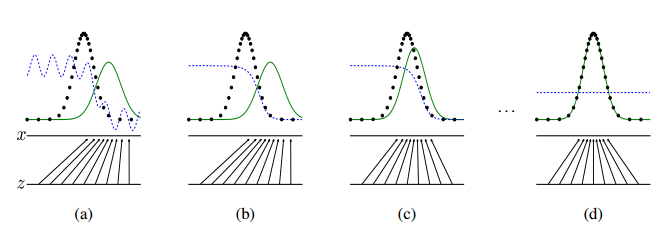
\includegraphics[width=0.7\textwidth]{img/distributions.png} 
\caption{Visualization of distributions/mapping $z\rightarrow x$,  \textit{Source: \textcircled{3}}}
\end{figure}

\vfill
} % END OF FRAME

%----------------------------------------

\section[Results and Evaluation]{Results and Evaluation}

\frame{
\frametitle{Training}
\begin{block}{\centering \textbf{Datasets}}
\begin{multicols}{2}
\begin{itemize}
	\item MNIST
	\item TFD: toronto face database
	\item CIFAR-10 [21] 
\end{itemize}
\end{multicols}
\end{block}

\begin{block}{\centering \textbf{Experiments}}\footnotesize
\begin{columns}
\begin{column}{.3\textwidth}
\textbf{Test scenario: }Estimation of propability of ''test set data'' under (behind) $p_g\rightarrow$ fit a Gaussian Parzen window to the samples generated with $G$ and report the log-likelihood considering test data samples obtaining variance $\sigma$ from cross-validation with the test dataset.
\end{column}
\begin{column}{.6\textwidth}
\begin{table}[T]
\begin{tabularx}{\textwidth}{X|X|X}
Model & MNIST & TFD\\
\toprule
DBN [3] & $138\pm 2$ & $1909\pm 66$\\
\hline 
Stacked CAE [3] & $121\pm 1.6$ & $2110\pm 50$\\
\hline 
Deep GSN [3] & $214\pm 1.1$ & $1890\pm 29$\\
\hline
GAN & $225\pm 2$ & $2057\pm 26$\\
\hline
\end{tabularx}
\caption{Log-likelihood estimates of $p_g$}
\end{table} 
\end{column}
\end{columns}
\end{block}} % END OF FRAME

\frame{
\frametitle{Sampling from the Model - 1}

\begin{figure}[t]
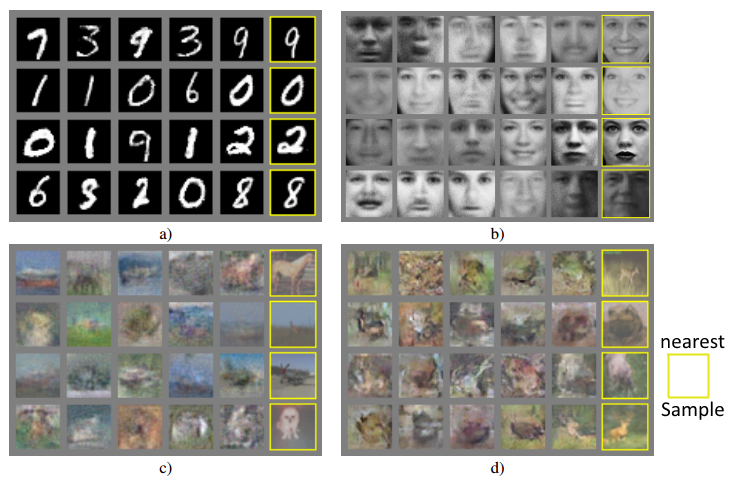
\includegraphics[width=0.5\textwidth]{img/samples_edit.PNG} 
\caption{Visualization of Samples from the model, \textit{Source: \textcircled{3}}}
\end{figure}

} % END OF FRAME
%----------------------------------------

\frame{
\frametitle{Sampling from the Model - 2}
\begin{block}{\centering \textbf{MNIST dataset}}
MNIST digits linearly interpolated to evaluate diversity of generative distribution $p_g$ of GAN approach..
\end{block}
\begin{figure}[t]

\includegraphics[width=0.7\textwidth]{img/digit_interpolation.PNG} 
\caption{Linearly interpolating digits in $z$-space of $G$ after training, \textit{Source: \textcircled{3}}}
\end{figure}

%\footnotetext{Goodfellow, Ian, et al. "Generative adversarial nets."}
} % END OF FRAME
%----------------------------------------

\frame{
\frametitle{Application in Biomedical Image Analysis}

\begin{columns}
\begin{column}{.5\textwidth}
\begin{block}{\centering \textbf{Application Example: Skin Lesion Segmentation}}
\begin{itemize}
\item Generator $G$: Fully (de-)convolutional neural network to synthesize (generate) valid segmentation masks
\item Discriminator $D$: another convolutional neural network to distinguish synthetic (fake) from real masks
\end{itemize}
\end{block}
\end{column}

\begin{column}{.5\textwidth}
\begin{figure}[t]
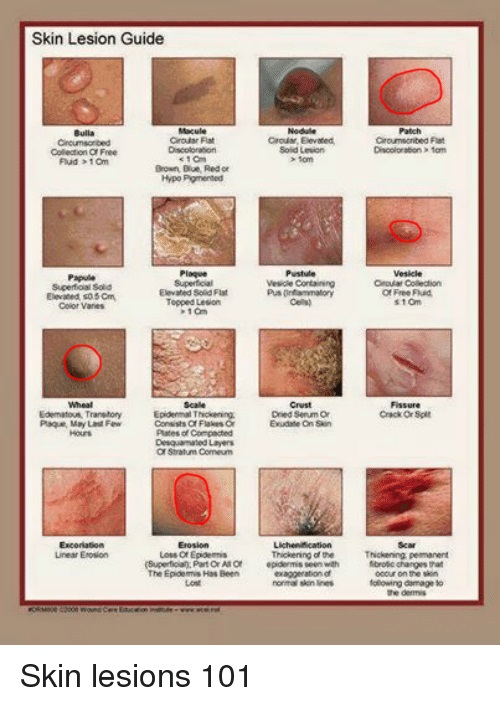
\includegraphics[width=0.5\textwidth]{img/lesions.jpg} 
\caption{Segmented Skin Lesions, \textit{Source: \footnotemark}}
\end{figure}
\end{column}
\end{columns}


\footnotetext{\url{https://suprememedical.com/Product/skin-lesion-guide}}
} % END OF FRAME
%----------------------------------------

\frame{
\frametitle{Benefits and Drawbacks}

\begin{block}{\centering \textbf{Advantages and Disadvantages}}
\begin{table}[T]
\begin{tabularx}{\textwidth}{X|X}
\textbf{\textcircled{+} Advantages} &  \textbf{\textcircled{-} Disadvantages}\\
\toprule
\tabitem no need for Markov Chains (MCMC-approaches)	 & \tabitem no explicit representation of $p_g(x)$\\
\tabitem training through standard backpropagation & \tabitem $D$ needs to be sufficiently synchronized with $G$ ($D$ must stay inline)\\
\tabitem incorporation of wide variety of functions possible $\rightarrow$ applicability\vskip 1pt {\tabitem able to represent sharp, degenerate distributions} & $\rightarrow$ avoidance of \emph{Helvetica scenario}: \vskip 5pt $G$ collapsing too many latent $z$'s (e.g. random variables) to the same sample $x$, leading to insufficient generative diversity\\
\hline
\end{tabularx}
\caption{Advantages and Disadvantages of GANs}
\end{table} 
\end{block}
%\footnotetext{Goodfellow, Ian, et al. "Generative adversarial nets."}
} % END OF FRAME
%----------------------------------------

\section[Conclusion and Future Work]{Conclusion and Future Work}

\frame{
\frametitle{Summary}

\begin{itemize}
\item GANs: new framework for estimating \alert{generative models} defined by multilayer perceptrons (Convolutional Layers) trained by standard backpropagation $\rightarrow$ no need for any Markov chains (MCMC-approaches), which can have problems Mixing (Converging)
\item Results\/ Samples considered to be \alert{competitive} with those of the state-of-the-art generative models
\item Empirical Evaluation (Fitting a Gaussian Parzen window to measure distribution similarity of $p_g$ as log-likelihood metric) indicates comparable scores than achieved for state-of-the-art methods like DBNs, Stacked CAE, GSN, Adversarial nets and \alert{comparable validity/representativity}
\end{itemize}
%\footnotetext{Goodfellow, Ian, et al. "Generative adversarial nets."}
} % END OF FRAME
%----------------------------------------

\frame{
\frametitle{Conclusion}

\begin{itemize}
\item approach is, besides DGMs (directed graphical models), the only one, inducing \alert{no problems} or further elaborations for sampling (generating samples) or training $\rightarrow$ rather simple implementation
\item experiments show \alert{comparable similarities} against state-of-the-art methods in log-likelhood score and variance in matching the prior distribution $p_z$ with the generative one ($p_g$), but the method proposed is regarded to be more simple than others
\item the \alert{synchronization of D} is yet an effortful factor, since sufficient reasoning for the number of steps of the inner loop is needed to avoid the previously named "Helvetica scenario"!
\item \alert{future applications} might involve the synthetic generation of morphologically correct segmentation masks of seperatable objects, fake images (databases), keys/passwords (cryptography), image processing
\end{itemize}

%\footnotetext{Goodfellow, Ian, et al. "Generative adversarial nets."}
} % END OF FRAME
%----------------------------------------

\frame{
\frametitle{Outlook}
\textbf{Straighforward extensions}:
\begin{enumerate}
\item Conditional generative Model $p(\mathbf{x}|c)$ w. adding condition $c$
\item Learned approximate inference: Predict prior-$z$ w. given latent $x$
\item Modeling of multiple Conditionals: $p(\mathbf{x}_S|\mathbf{x}_\xout{S})$
\item Semi-Supervised Learning: Better Performance w. partially labeled training data
\item Efficiency improvements: Better methods to coordinate $G$ and $D$, better distributions to sample $z$ from during training
\end{enumerate}

%\footnotetext{Goodfellow, Ian, et al. "Generative adversarial nets."
} % END OF FRAME
%----------------------------------------

%========================================

%\frame{
%\frametitle{Vor - Nachteile}
%
%\begin{columns}[b]
%\begin{column}{.5\textwidth}
%{\color{unirot}Vorteile}
%\begin{itemize}
%  \item da gibt es viele
%  \item und noch mehr
%  \item und immer mehr
%  \item und ein letzter Vorteil
%\end{itemize}
%\end{column}
%
%
%\begin{column}{.5\textwidth}
%{\color{unirot}Nachteile} 
%\begin{itemize}
%  \item da gibt nur einen
%  \item oder zwei
%\end{itemize}
%\end{column}
%
%\end{columns}
%\vfill
%} % END OF FRAME


%========================================
%========================================
%========================================

% hilights mit \alert oder \hilite




%----------------------------------------

\frame{\frametitle{Questions?}
\begin{figure}

\includegraphics[width=.8\textwidth]{img/questions} 
\end{figure}
\vspace*{-3.3cm}\begin{center}\begin{LARGE}\textbf{Questions?}\end{LARGE}\end{center}

\vspace*{2cm}
}

\frame{
\frametitle{Sources and further reading}
\begin{block}{\centering \textbf{Literature}}
\small
\begin{enumerate}
\item Goodfellow, Ian, et al. "Generative adversarial nets."
\item Izadi, Saeed \& Mirikharaji, Zahra \& Kawahara, Jeremy \& Hamarneh, Ghassan. Generative adversarial networks to segment skin lesions.
\end{enumerate}
\end{block}
\begin{block}{\centering \textbf{Images}}
\small
\begin{enumerate}
\item {\url{https://www.sevendaysvt.com/vermont/some-counterfeiters-still-do-it-old-school/Content?oid=3276910}}
\item \small \url{https://www.altoros.com/blog/the-diversity-of-tensorflow-wrappers}\\ \url{-gpus-generative-adversarial-networks-etc/} \& \url{https://medium.freecodecamp.org/an-intuitive-introduction-to-generative}\\ \url{-adversarial-networks-gans-7a2264a81394}
\item Goodfellow, Ian, et al. "Generative adversarial nets."

\end{enumerate}
\end{block}
}


\end{document}
